\documentclass{standalone}
\usepackage{pgfplots}
\begin{document}
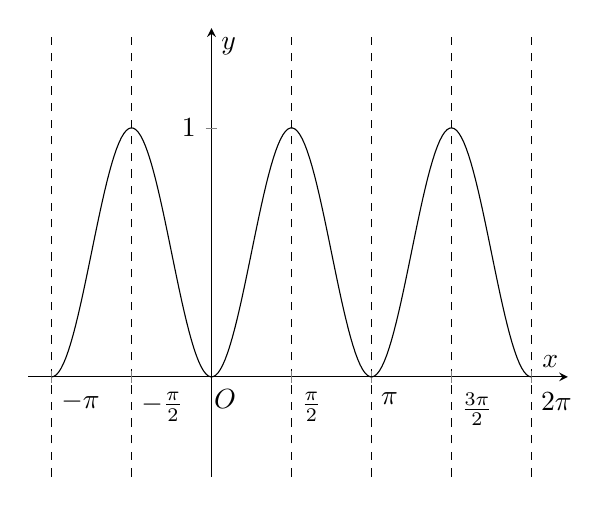
\begin{tikzpicture}
\begin{axis}
[
ymin=-0.4,ymax=1.4,
xmin=-3.6,xmax=7,
xtick=\empty,
ytick=\empty,
extra x ticks={-3.14159, -1.5708, 1.5708, 3.14159, 4.71239, 6.28319},
extra x tick labels={$-\pi$, $-\frac{\pi}{2}$, $\frac{\pi}{2}$, $\pi$, $\frac{3\pi}{2}$, $2\pi$},
extra y ticks={1},
extra y tick labels={$1$},
every extra x tick/.style={
    xticklabel style={anchor=north west},
    grid=major,
    major grid style={very thin,dashed,black}
},
axis lines = center,
xlabel=$x$,ylabel=$y$,
samples=200,
]
\addplot [black, domain=-3.14159:6.28319] {(sin(deg(x)))^2};
\node at (axis cs:0.265, -0.09) {$O$} ;
\end{axis}
\end{tikzpicture}
\end{document}
